\documentclass[ngerman]{beamer}
\usepackage{mathptmx}
\usepackage[T1]{fontenc}
\usepackage[utf8]{inputenc}
\usepackage{babel}
\usepackage{amsmath}
\usepackage{amssymb}
\usepackage{graphicx}
\usetheme{Warsaw}
\setbeamercovered{transparent}
%\setbeamertemplate{footline}[frame number]

\title{Praxisprojekt}
\subtitle{Fortschritte \\
	Aktuelle Folie: \ref{Aktuelle Folie}}
\author[J.~Dielmann]{Johannes~Dielmann\inst{1}}
\institute{
	\inst{1}Mess- und Sensortechnik\\
	RheinAhrCampus}
\date{\today}
\subject{Praxisprojekt}
\keywords{Praxisprojket, Mikroncontroller, C, Schrittmotor, 3D-Laserscanner}


\begin{document}
\titlepage

\pgfdeclareimage[height=0.5cm]{institution-logo}{./_Res/RAC_Logo}
\logo{\pgfuseimage{institution-logo}}

\frame{
	\frametitle{Gliederung} 
	\tableofcontents[subsectionstyle=show/shaded/hide]
}

\section{Oktober}
\subsection{1. Woche}
\begin{frame}\frametitle{03.10.2011 - 09.10.2011}
\begin{itemize}
	\item Inbetriebnahme der Stepper-Karte 
	\begin{itemize}
		\item Ansteuerung mittels Hyperterminal 
	\end{itemize}
	
	\item Inbetriebnahme des STK500 Microkontrollerboard 
	\begin{itemize}
		\item Kleine Programme zum Testen der LEDs und Taster 
		\item Bibliothek zum entprellen der Taster eingebunden 
		\item UART Schnittstelle aktiviert
	\end{itemize}
\end{itemize}
\end{frame}
\subsection{2. Woche}
\begin{frame}\frametitle{10.10.2011 - 16.10.2011}
Erledigt:
\begin{itemize}
\item Verbindung zwischen Mikrocontroller und Stepper-Karte 
\item Hinzufügen eines Displays 
\item Inbetriebnahme des VI-900 Lasererfassungsystem 
\item Programm auf kompletten Befehlssatz erweitern 
\item Statusmeldungen auf Display ausgeben 
\item Vollständige Steuerung über Taster/Display (Menü) 
\end{itemize}
Probleme: 
\begin{itemize}
\item Mikrocontroller hat keine 2. Schnittstelle Multipl.? Software Uart? 
\begin{itemize}
\item Abgelehnt Anderer Mikrocontroller! 2x UART + 3 Interrupt 
\end{itemize}
\item Defekte Menü Bibliothek 
\end{itemize}
Offene Ziele: 
\begin{itemize}
\item 2. Karte in Betrieb nehmen und Endschalter verbinden 
\item Protokoll abhören
\end{itemize}
\end{frame}
\subsection{3. Woche}
\begin{frame}\frametitle{17.10.2011 - 23.10.2011}
Erledigt: 
\begin{itemize}
\item Protokoll in Erfahrung bringen 
\item Protokoll in groben Zügen adaptiert 
\end{itemize}
In Bearbeitung: 
\begin{itemize}
\item Anderen Mikrocontroller besorgen 
\item Lizenz (neue angefordert) 
\item 2. Karte in Betrieb nehmen und Endschalter verbinden 
\item Auftrag an Werkstatt gegeben (ca. 2 Wochen) 
\end{itemize}
Zu erledigen: 
\begin{itemize}
\item Gedrehtes Pin-Pin Kabel bauen 
\item Normales Serielles Kabel bauen (min. 6m) 
\item Keine 9 Pol. Kabel in Werkstatt 
\end{itemize}
Nicht mehr relevant:
\begin{itemize}
\item Menü austauschen (zu Speicherintensiv)
\end{itemize}
\end{frame}
\subsection{4. Woche}
\begin{frame}\frametitle{27.10.2011 - 03.11.2011}
Erreicht: 
\begin{itemize}
\item MAX232 auf Steckboard vorbereiten (2. Schnittstelle) 
\item Überall Richtige Buchsen/Stecker verbauen 
\item Protokoll für Rapidform Motoren anpassen (verbessern) 
\item 2. Karte in Betrieb genommen 
\item Begonnen Endschalter anzuschliessen 
\end{itemize}
Probleme: 
\begin{itemize}
\item Warten auf neuen Mikrocontroller (heute oder morgen) 
\item Warten auf 2. Platine aus Werkstatt (workaround) 
\item Speicherplatz auf Mikrocontroller zu gering (neuer) 
\end{itemize}
Nicht erreichte Ziele: 
\begin{itemize}
\item Platinenlayout mit Eagle erstellen 

\begin{itemize}
\item 2-RS; 2 Max 232; Pinheader Drehgeber; Pinheader Display 
\end{itemize}
\item Einschubfront Planen (LCD; Drehgeber; 2 D-Sub)
\end{itemize}
\end{frame}
\section{November}
\subsection{5. Woche}
\begin{frame}\frametitle{04.11.2011 - 10.10.2011}
Erledigt: 
\begin{itemize}
\item Prorgamm auf neuen Mikrocontroller anpassen 
\item Auf externen Max232 gewechselt 
\item Motor Platinen komplett fertig gestellt 
\end{itemize}
Probleme: 
\begin{itemize}
\item Falscher Mikrocontroller geliefert neuer Bestellt (Fr. o. Mo.) 
\item Anpassung auf neuen Mikrocontroller war problematisch 
\item Programmierung nur noch über AVRISPmkII 
\item Falsche Fuses gesetzt (JTAG, Watchdog, CKPSC, CKSRC) 
\item Register haben neue Namen 
\item Endschalter haben zu geringen Schaltabstand neue Endschalter
\end{itemize}
Offene Ziele: 
\begin{itemize}
\item Beide Schnittstellen in Betrieb nehmen 
\item Endschalter am Mikrocontroller berücksichtigen 
\end{itemize}
\end{frame}
\subsection{6. Woche}
\begin{frame}\frametitle{11.11.2011 - 17.11.2011}
Erledigt: 
\begin{itemize}
\item Endschalter verdrahtet (In Motorkabel integriert) 
\item Neuer Mikrocontroller eingetroffen 
\end{itemize}
Probleme: 
\begin{itemize}
\item Beschaltung der Endschalter war unklar 
\item Defekter Optokoppler 
\item Mikrocontroller startet, bei Timer überlauf, ständig neu 
\end{itemize}
Verworfene Ziele: 
\begin{itemize}
\item Neue Endschalter besorgen
\end{itemize}
Nicht erreichte Ziele: 
\begin{itemize}
\item Beide Schnittstellen in Betrieb nehmen 
\item Endschalter am Mikrocontroller beruecksichtigen 
\item Eagle Layout beginnen
\end{itemize}
\end{frame}
\subsection{7. Woche}
\begin{frame}\frametitle{18.11.2011 - 25.11.2011}
Offene Ziele: 
\begin{itemize}
\item Programm an Mikrocontroller anpassen 
\item 2 Schnittstellen in Betrieb nehmen 
\item Endschalter richtig verdrahten
\end{itemize}
\end{frame}
\subsection{8. Woche}
\begin{frame}\frametitle{26.11.2011 - 01.12.2011}
Erreichte Ziele: 
\begin{itemize}
\item Programm an Mikrocontroller anpassen 

\begin{itemize}
\item Defekte Bibliothek von Atmel 
\end{itemize}
\item Vollständiger Wechsel zu Eclipse/AVRDude 
\item 2 Schnittstellen in Betrieb nehmen 

\begin{itemize}
\item Größtenteils Vollständig 
\end{itemize}
\item Funktionsfähige ISR um Motor zu stoppen 
\item Endschalter richtig verdrahten
\end{itemize}
\end{frame}
\section{Dezember}
\subsection{9. Woche}
\begin{frame}\frametitle{02.12.2011 - 08.12.2011}
Erreichte Ziele: 
\begin{itemize}
\item Programmablauf optimiert (Vollständige Steuerung durch Software, weitere
Protokolle integriert) 
\item Quellcode auf Github hoch geladen (https://github.com/JoeD84/Praxisprojekt) 
\item Automatische Protokollauswahl (incl. Terminal) 
\item Beide Endschalter funktionieren problemlos 
\item Platinen Layout begonnen 
\item Motor einstellungen optiemiert (100.000 Schritte / Umdrehung. Umrechnungsfaktoren
angepasst) 
\end{itemize}
Nicht erreichte Ziele: 
\begin{itemize}
\item Platine ätzen lassen 
\item Vollständige Bilderserie aufnehmen
\end{itemize}
\end{frame}
\subsection{10. Woche}
\begin{frame}\frametitle{09.12.2011 - 14.12.2011}
Ziele: 
\begin{itemize}
\item Platinenlayout fertigstellen und ätzen lassen (mit KiCad) 
\item Praxisbericht schreiben (mit \LaTeX{}) 
\item 3D Objekt vollständig aufnehmen
\end{itemize}
\end{frame}
\subsection{11. Woche}
\begin{frame}\frametitle{15.12.2011 - 22.12.2011}
\label{Aktuelle Folie}
Erreichte Ziele:
\begin{itemize}
\item Umstellung der Präsentation auf \LaTeX{}
\item Praxisbericht begonnen
\item Vollständige Aufnahme eines 3D Objektes und manuelles zusammenfügen
des Objektes
\end{itemize}
Nicht erreichte Ziele:
\begin{itemize}
\item Platinenlayout ätzen lassen (Erst ab 9. Januar)
\end{itemize}
\end{frame}
\begin{frame}\frametitle{15.12.2011 - 22.11.2011}
\framesubtitle{3D Objekt}
\begin{itemize}
\item 
\begin{figure}
\caption{\protect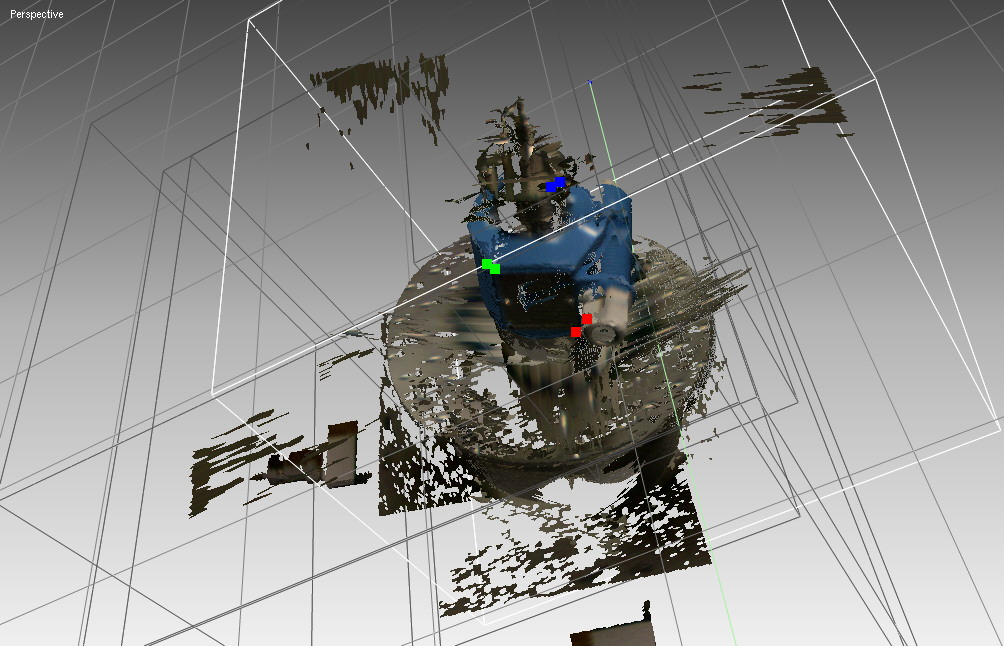
\includegraphics[scale=0.5]{./_Res/Motor_vollstaendig_schlecht}}
\end{figure}

\end{itemize}
\end{frame}
\subsection{12. Woche}
\begin{frame}\frametitle{23.12.2011 - 01.2012}
Ziele:
\begin{itemize}
	\item Platinenlayout ätzen lassen
	\item Praxisbericht fertigstellen
\end{itemize}
\end{frame}

\end{document}
